\documentclass{standalone}
\usepackage{tikz}
\begin{document}
\scriptsize
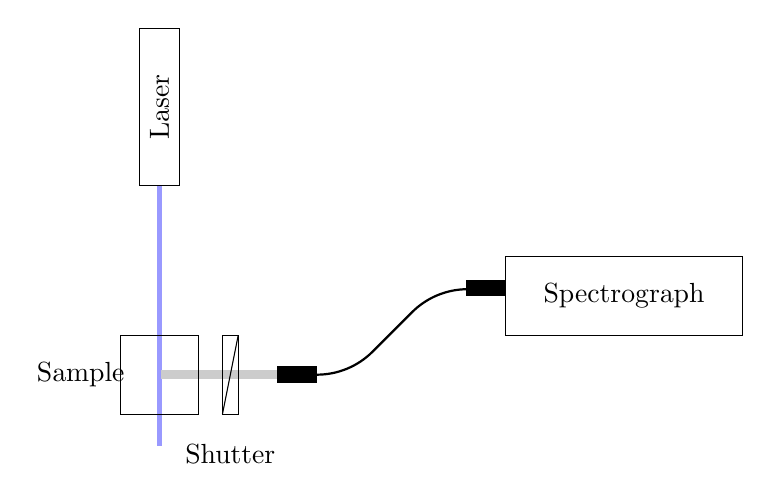
\begin{tikzpicture}
  \draw[draw=blue!40,fill=blue!40] (6.475,4) rectangle (6.525,0.7);
  \draw[draw=black!20,fill=black!20] (6.525,1.55) rectangle (8,1.65);
  %
  \draw (6,1.1) rectangle ++(1,1);
  \draw (5.5,1.6) node {Sample};
  %
  \draw (7.3,1.1) rectangle ++(0.2,1);
  \draw (7.3,1.1) -- ++(0.2,1);
  \draw (7.4,0.6) node {Shutter};
  %
  \draw[fill] (8,1.5) rectangle ++(0.5,0.2);
  \draw[thick] (8.5,1.6) arc (-90:-45:1) -- ++(0.5,0.5) arc (135:90:1);
  \draw[fill] (10.4,2.6) rectangle ++(0.5,0.2);
  %
  \draw (10.9,2.1) rectangle ++(3,1);
  \draw (12.4,2.6) node {Spectrograph};
  %
  \draw (6.25,4) rectangle ++(0.5,2);
  \draw (6.5,5) node [rotate=90] {Laser};
  %
\end{tikzpicture}
\end{document}
